\documentclass[]{beamer}
\usepackage[T1]{fontenc}
\usepackage[utf8]{inputenc}
\usepackage{lmodern}
\usepackage[italian]{babel}
\usepackage{mathrsfs}
\usepackage{cancel}





\title{Vettori e operazioni sui vettori}
\author{\texorpdfstring{Mattia Cozzi\newline\href{mailto:cozzimattia@gmail.com}{\texttt{cozzimattia@gmail.com}}}{Mattia Cozzi}}
\date{a.s.~2023/2024}
%\documentclass[handout]{beamer}     %usare questa classe per generare l'handout
%\usepackage{pgfpages}   %per mostrare più quadri nella stessa pagina
%\pgfpagesuselayout{4 on 1}[a4paper,border shrink=5mm,landscape]
\usetheme{Singapore}
%\useoutertheme[left]{sidebar} %elementi intorno alle diapositive
\setbeamercovered{dynamic} %modifica l'aspetto del testo grigetto delle diapositive future. Argomenti: invisible/transparent/dynamic

\usecolortheme{orchid}





\theoremstyle{plain}
\newtheorem{teorema}{Teorema}

\usepackage{tikz}
\usepackage{circuitikz}

\usepackage{pgf,pgfplots,graphicx}
\usetikzlibrary{angles,quotes,arrows,shapes,decorations.markings}
\pgfplotsset{compat=1.15}
\usepgfplotslibrary{units,fillbetween} % to add units easily to axis

\newcommand{\fem}{f_{em}}

\def\angolo[#1](#2)(#3:#4:#5)% Syntax: [draw options] (center) (initial angle:final angle:radius)
    { \draw[#1] ($(#2)+({#5*cos(#3)},{#5*sin(#3)})$) arc (#3:#4:#5); }


\begin{document}

\begin{frame}
  \titlepage
\end{frame}





\begin{frame}
\frametitle{Contenuti}
\tableofcontents
\end{frame}


\section{Vettori}


\begin{frame}
  \frametitle{Scalari e vettori}
  In fisica, una grandezza può:
\begin{itemize}
  \item essere espressa completamente tramite un valore numerico, come la massa o la temperatura: è uno \alert<1,3>{scalare};\pause
  \item richiedere l'esplicitazione anche di una \emph{direzione} e di un \emph{verso}, come la velocità o la forza: è un \alert<2-3>{vettore}.\pause
\end{itemize}

~

  Gli scalari sono indicati con lettere, i vettori con lettere sormontate da una freccia, come $ \vec{a} $.\pause
  
  ~
  
  Il modulo del vettore $ \vec{a} $ viene indicato con $ |\vec{a}| $ o più semplicemente con $ a $.
\end{frame}

\begin{frame}
\frametitle{Caratteristiche di un vettore (1)}
  Un vettore \emph{viene rappresentato come una freccia} (ma non \emph{è} una freccia!) in cui:
  \begin{itemize}
    \item la lunghezza della freccia indica il \alert{modulo/intensità} del vettore ed è indicata tramite un \textcolor{blue}{numero} (uno scalare);\pause
    \item la retta sulla quale giace la freccia è la \alert{direzione} del vettore ed è indicata mediante l'\textcolor{blue}{angolo} formato con l'asse $ x $;\pause
    \item l'orientamento della freccia sulla sua direzione indica il \alert{verso} del vettore e viene indicato con un \textcolor{blue}{segno} $ + $ o $ - $. 
  \end{itemize}
\end{frame}



\begin{frame}
\frametitle{Caratteristiche di un vettore (2)}
\begin{figure}
\begin{tikzpicture}[scale=1.5]
\angolo[magenta](0,0)(0:60:.5)
\draw [dashed] (-1,0) -- (1,0);
\draw [thick,orange,dashed] (3*.5,3*.866) -- (-1*.5,-1*.866);
\draw [thick] (0,0) circle [radius=.01];
\draw [->,thick,blue] (0,0) -- (2*.5,2*.866);
\node [right,blue] at (.6,.9) {{\scriptsize $ \vec{v} $}};
\node [left] at (.3,1) {{\scriptsize modulo di $ \vec{v} $ = $ |\vec{v}| $ = $ v $}};
\node [above,magenta] at (.5,.2) {{\scriptsize $ \theta $}};
\draw [|<->|] (1-.2*.866,2*.866+.2*.5) -- (-.2*.866,.2*.5);
\node [below] at (-1.5,0) {{\scriptsize linea di riferimento $ r $}};
\node [left,orange] at (3*.5,3*.866) {{\scriptsize direzione}};
\end{tikzpicture}
\end{figure}
\end{frame}


\begin{frame}
  \frametitle{Versori}
  Un versore è un \alert{vettore di modulo $ 1 $} e viene indicato con $ \hat{a} $, $ \hat{b} $, ecc.{\pause} 
  
  ~
  
  Solitamente i versori $ \hat{i}  $, $ \hat{j} $ e $ \hat{k} $ sono usati per indicare gli assi cartesiani\footnote{Ma si usano anche $ \hat{x} $, $ \hat{y} $ e $ \hat{z} $.}.
  
  \begin{figure}
  \begin{tikzpicture}[scale=1]
  \draw[->] (-.5,0) -- (4,0);
  \draw[->] (0,-.5) -- (0,3);
  \draw[->] (-.4,-.2) -- (3,1.5);
  \draw[->,red,thick] (0,0) -- (1,0);
  \draw[->,red,thick] (0,0) -- (0,1);
  \draw[->,red,thick] (0,0) -- (.8,.4);
  \node [below] at (4,0) {$ x $};
  \node [below,red] at (.5,0) {$ \hat{i} $};
  \node [left,red] at (0,.5) {$ \hat{j} $};
  \node [above,red] at (.4,.2) {$ \hat{k} $};
  \node [left] at (0,3) {$ y $};
  \node [above] at (3,1.5) {$ z $};
  \end{tikzpicture}
  \end{figure}
\end{frame}




\begin{frame}
  \frametitle{Scrittura cartesiana di un vettore}
  Sfruttando i versori, possiamo facilmente esprimere un versore in \emph{forma cartesiana}.
  
  \begin{figure}
  \begin{tikzpicture}[scale=1]
  \draw[dashed,gray] (-2,2) -- (3,2);
  \draw[dashed,gray] (3,0) -- (3,2);
  \draw[dashed,gray] (-2,0) -- (-2,2);
  \draw[->] (-3,0) -- (4,0);
  \draw[->] (0,-.5) -- (0,3);
  \draw[->,red,thick] (0,0) -- (1,0);
  \draw[->,red,thick] (0,0) -- (0,1);
  \node[below] at (4,0) {$ x $};
  \node[below,red] at (.5,.1) {\small $ \hat{i} $};
  \node[left,red] at (.1,.5) {{\small $ \hat{j} $}};
  \node[left] at (0,3) {$ y $};
  \node[above,cyan] at (-1,1.2) {$ \vec{b} $};
  \node[above,blue] at (1.5,1.2) {$ \vec{a} $};
  \draw[->,blue,thick] (0,0) -- (3,2);
  \draw[->,cyan,thick] (0,0) -- (-2,2);
  \draw[] (-2,-.1) -- (-2,.1);
  \draw[] (3,-.1) -- (3,.1);
  \draw[] (.1,2) -- (-.1,2);
  \node[below] at (-2,0) {$ -2 $};
  \node[below] at (3,0) {$ 3 $};
  \node[left] at (0,2) {$ 2 $};
  \node[below,cyan] at (-2,-.5) {$ \vec{b} = -2\hat{i} + 2\hat{j} $};
  \node[below,blue] at (2,-.5) {$ \vec{a} = 3\hat{i} + 2\hat{j} $};
  \end{tikzpicture}
  \end{figure}
\end{frame}


\section{Scomposizione}


\begin{frame}
  \frametitle{Le funzioni trigonometriche}
Per lavorare con i vettori sono essenziali le funzioni goniometriche di \emph{seno}, \emph{coseno} e \emph{tangente}, definite come:



\begin{columns}
\begin{column}{0.5\textwidth}

  \begin{figure}
  \begin{tikzpicture}[scale=1]
  \draw (0,0) -- (4,0);
  \node [below] at (2,0) {$ c_{adj} $};
  \draw (4,0) --(4,3);
  \node [right] at (4,1.5) {$ c_{opp} $};
  \draw (4,3) -- (0,0);
  \node [above left] at (2,1.5) {$ i $};
  \draw (0.4,0) arc [start angle=0,end angle=37,radius=0.4] node[pos=0.8,right]{$\theta$};
  \end{tikzpicture}
  \end{figure}

\end{column}
\begin{column}{0.5\textwidth}

\begin{center}
\colorbox{blue!30}{$ \sin\theta = \dfrac{c_{opp}}{i} $}\\~\\
\colorbox{blue!30}{$ \cos\theta = \dfrac{c_{adj}}{i} $}\\~\\
\colorbox{blue!30}{$ \tan\theta = \dfrac{c_{opp}}{c_{adj}} $}
\end{center}
Essendo $ i $ sempre maggiore dei cateti, i valori di seno e coseno non possono essere maggiori di $ 1 $.
\end{column}
\end{columns}
\end{frame}






\begin{frame}
  \frametitle{Scomposizione di un vettore}
  Una volta stabilito un sistema di riferimento, possiamo determinare l'angolo $ \theta $ che un vettore $ \vec{a} $ forma con l'asse $ x $ (la cui direzione è data dal versore $ \hat{i} $) e calcolare le \alert{componenti cartesiane} del vettore (ovvero le sue \emph{proiezioni sugli assi} cartesiani).


\begin{figure}
\begin{tikzpicture}[scale=1.5]
\angolo[](0,0)(0:33:.5)
\draw (-.5,0) -- (0,0) -- (0,-.5);
\draw [dashed] (3,2) -- (3,0);
\draw [dashed] (3,2) -- (0,2);
\draw [<->] (0,3) -- (0,0) -- (4,0);
\draw [thick] (0,0) circle [radius=.01];
\draw [->,thick,cyan] (0,0) -- (3,2);
\draw [->,thick,blue] (0,0) -- (0,2);
\draw [->,thick,blue] (0,0) -- (3,0);
\node [right,cyan] at (.6,.9) {{\scriptsize $ \vec{a} $}};
\node [left,red] at (0,.5) {{\scriptsize $ \hat{j} $}};
\node [below,red] at (.5,0) {{\scriptsize $ \hat{i} $}};
\node [left] at (0,3) {{\scriptsize $ y $}};
\node [left,blue] at (0,1) {{\scriptsize $ a_y $}};
\node [below] at (4,0) {{\scriptsize $ x $}};
\node [below,blue] at (1.5,0) {{\scriptsize $ a_x $}};
\node [above] at (.65,.08) {{\scriptsize $ \theta $}};
\draw [->,thick,red] (0,0) -- (1,0);
\draw [->,thick,red] (0,0) -- (0,1);
\end{tikzpicture}
\end{figure}
\end{frame}

\begin{frame}
  \frametitle{Scomposizione di un vettore (2)}
  \begin{figure}
\begin{tikzpicture}[scale=.6]
\angolo[](0,0)(0:33:.5)
\draw (-.5,0) -- (0,0) -- (0,-.5);
\draw [dashed] (3,2) -- (3,0);
\draw [dashed] (3,2) -- (0,2);
\draw [<->] (0,3) -- (0,0) -- (4,0);
\draw [thick] (0,0) circle [radius=.01];
\draw [->,thick,cyan] (0,0) -- (3,2);
\draw [->,thick,blue] (0,0) -- (0,2);
\draw [->,thick,blue] (0,0) -- (3,0);
\node [right,cyan] at (.6,1) {{\scriptsize $ \vec{a} $}};
\node [left] at (0,3) {{\scriptsize $ y $}};
\node [left,blue] at (0,1) {{\scriptsize $ a_y $}};
\node [below] at (4,0) {{\scriptsize $ x $}};
\node [below,blue] at (1.5,0) {{\scriptsize $ a_x $}};
\end{tikzpicture}
\end{figure}
  Calcoliamo le \alert{componenti cartesiane} del vettore (ovvero le sue \emph{proiezioni sugli assi} cartesiani) utilizzando le formule precedenti:
\begin{center}
\colorbox{blue!30}{ $ a_x = a  \cos\theta  $} e \colorbox{blue!30}{ $ a_y = a  \sin\theta  $}
\end{center}\pause
~\\
Possiamo anche esprimere il vettore $ \vec{a} $ in \emph{forma cartesiana}:
\begin{center}
\colorbox{blue!30}{ $ \vec{a} = a_x \hat{i} + a_y \hat{j} $ }
\end{center}
\end{frame}

\begin{frame}
  \frametitle{Esempio 1}


\begin{figure}
\begin{tikzpicture}[scale=.8]
\angolo[](0,0)(0:120:.5)
\draw (-3,0) -- (0,0) -- (0,-1);
\draw [dashed] (-3*.5,3*.866) -- (0,3*.866);
\draw [dashed] (-3*.5,3*.866) -- (-3*.5,0);
\draw [<->] (0,4) -- (0,0) -- (2,0);
\draw [thick] (0,0) circle [radius=.01];
\draw [->,thick,cyan] (0,0) -- (-3*.5,3*.866);
\draw [->,thick,blue] (0,0) -- (-3*.5,0);
\draw [->,thick,blue] (0,0) -- (0,3*.866);
\node [right,cyan] at (2*-.6,2*1) {{\scriptsize $ \vec{a} $}};
\node [right,cyan] at (1,2.5) {{\scriptsize $ a = 3 $}};
\node [left] at (0,4) {{\scriptsize $ y $}};
\node [right,blue] at (0,1.5*.866) {{\scriptsize $ a_y $}};
\node [right] at (.4,.4) {{\scriptsize $ \theta =120^\circ $}};
\node [below] at (2,0) {{\scriptsize $ x $}};
\node [below,blue] at (-1.5*.5,0) {{\scriptsize $ a_x $}};
\end{tikzpicture}
\end{figure}\pause


\begin{center}
$ a_x = 3 \cdot \cos(120^\circ) = 3 \cdot \left(-0,5\right) = - 1,5$

~

$ a_y = 3 \cdot \sin(120^\circ) = 3 \cdot \left(0,866\right) =  2,6$

~

$ \vec{a}= -1,5\hat{i} + 2,6\hat{j} $
\end{center}
\end{frame}

\begin{frame}
\frametitle{Esercizio}
\begin{exampleblock}{Calcolo delle componenti}
  Sapendo che il vettore $ \vec{a} $ ha modulo $ 10 $ e forma con l'asse delle $ x $ un angolo di $ 70^\circ $, esprimi $ \vec{a} $ in forma cartesiana.
\end{exampleblock} 
\end{frame}


\begin{frame}
  \frametitle{Modulo e componenti di un vettore}
  \begin{figure}
\begin{tikzpicture}[scale=.6]
\angolo[](0,0)(0:33:.5)
\draw (-.5,0) -- (0,0) -- (0,-.5);
\draw [dashed] (3,2) -- (3,0);
\draw [dashed] (3,2) -- (0,2);
\draw [<->] (0,3) -- (0,0) -- (4,0);
\draw [thick] (0,0) circle [radius=.01];
\draw [->,thick,cyan] (0,0) -- (3,2);
\draw [->,thick,blue] (0,0) -- (0,2);
\draw [->,thick,blue] (0,0) -- (3,0);
\node [right,cyan] at (.6,1) {{\scriptsize $ \vec{a} $}};
\node [left] at (0,3) {{\scriptsize $ y $}};
\node [left,blue] at (0,1) {{\scriptsize $ a_y $}};
\node [below] at (4,0) {{\scriptsize $ x $}};
\node [below,blue] at (1.5,0) {{\scriptsize $ a_x $}};
\end{tikzpicture}
\end{figure}
  Conoscendo le componenti $ a_x $ e $ a_y $ di un vettore $ \vec{a} $, è possibile risalire al suo modulo con il teorema di Pitagora:
  \begin{center}
\colorbox{blue!30}{ $ a = \sqrt{a_x^2 + a_y^2} $ }
\end{center}
\end{frame}


\begin{frame}
  \frametitle{Esempio 2}


\begin{figure}
\begin{tikzpicture}[scale=.7]
\angolo[](0,0)(0:120:.5)
\draw (-3,0) -- (0,0) -- (0,-1);
\draw [dashed] (-3*.5,3*.866) -- (0,3*.866);
\draw [dashed] (-3*.5,3*.866) -- (-3*.5,0);
\draw [<->] (0,4) -- (0,0) -- (2,0);
\draw [thick] (0,0) circle [radius=.01];
\draw [->,thick,cyan] (0,0) -- (-3*.5,3*.866);
\draw [->,thick,blue] (0,0) -- (-3*.5,0);
\draw [->,thick,blue] (0,0) -- (0,3*.866);
\node [right,cyan] at (2*-.6,2*1) {{\scriptsize $ \vec{a} $}};
\node [left] at (0,4) {{\scriptsize $ y $}};
\node [right,blue] at (0,1.5*.866) {{\scriptsize $ 2,6 $}};
\node [right] at (.4,.4) {{\scriptsize $ \theta $}};
\node [below] at (2,0) {{\scriptsize $ x $}};
\node [below,blue] at (-1.5*.5,0) {{\scriptsize $ -1,5 $}};
\end{tikzpicture}
\end{figure}


\begin{center}
$ a = \sqrt{(-1,5)^2 + (2,6)^2} = 3 $
\end{center}
\end{frame}


\begin{frame}
\frametitle{Dalla forma cartesiana alla polare}
Un vettore è espresso in \alert<1>{forma polare} quando se ne conoscono il modulo e l'angolo che esso forma con l'asse delle ascisse.\pause

~

Se conosciamo le componenti del vettore, possiamo conoscere il seno, il coseno o la tangente dell'angolo che esso forma con l'asse $ x $, e così facendo risalire al valore dell'angolo.\pause

~

L'angolo si trova utilizzando le funzioni inverse delle funzioni goniometriche:
\begin{center}
$ \alpha = \arcsin \left( \dfrac{a_y}{a} \right) = \arccos \left( \dfrac{a_x}{a} \right) = \arctan \left( \dfrac{a_y}{a_x} \right) = 61^{\circ} $
\end{center}
\end{frame}

\begin{frame}
\frametitle{Esercizio}
\begin{exampleblock}{Forma polare di un vettore}
È dato il vettore:
  \begin{center}
    $ \vec{a} = 3,2\hat{i} + 1,8\hat{j} $.
  \end{center}
Trova il modulo di $ \vec{a} $ e l'angolo che esso forma con l'asse delle ascisse.
\end{exampleblock} 
\end{frame}


\begin{frame}
  \frametitle{Assi cartesiani ``strani''}
  A volte ci troveremo a lavorare con assi cartesiani disposti diversamente dal modo usuale (ma comunque perpendicolari tra loro):
  
\begin{columns}
\begin{column}{0.3\textwidth}

\begin{figure}
\begin{tikzpicture}[scale=.6]
\draw [->,thick,cyan] (0,0) -- (-3,-2);
\draw [->,thick,cyan] (0,0) -- (-2,3);
\node [below,cyan] at (-3,-2) {{\scriptsize $ x $}};
\node [above,cyan] at (-2,3) {{\scriptsize $ y $}};
\end{tikzpicture}
\end{figure}

\end{column}
\begin{column}{0.3\textwidth}

\begin{figure}
\begin{tikzpicture}[scale=.6]
\draw [->,thick,red] (0,0) -- (-4,0);
\draw [->,thick,red] (0,0) -- (0,4);
\node [below,red] at (-4,0) {{\scriptsize $ x $}};
\node [right,red] at (0,4) {{\scriptsize $ y $}};
\end{tikzpicture}
\end{figure}

\end{column}
\begin{column}{0.3\textwidth}

\begin{figure}
\begin{tikzpicture}[scale=.6]
\draw [->,thick,olive] (0,0) -- (4,0);
\draw [->,thick,olive] (0,0) -- (0,-4);
\node [above,olive] at (4,0) {{\scriptsize $ x $}};
\node [left,olive] at (0,-4) {{\scriptsize $ y $}};
\end{tikzpicture}
\end{figure}

\end{column}
\end{columns}
\end{frame}


\begin{frame}
  \frametitle{Scomposizioni diverse a seconda degli assi}
  La disposizione degli assi avrà effetto sul modo in cui scomporremo un vettore: orientando diversamente gli assi, uno stesso vettore avrà \alert{componenti diverse}, eventualmente con \alert{segno diverso}\footnote{Diremo che il vettore è un \emph{invariante}, mentre non lo sono le sue componenti, che dipendono dagli assi.}.
\begin{columns}
\begin{column}{0.4\textwidth}

\begin{figure}
\begin{tikzpicture}[scale=.6]
\angolo[->](0,0)(212:152:.4)
\draw [->,thick,cyan] (0,0) -- (-3,-2);
\draw [->,thick,cyan] (0,0) -- (-2,3);
\draw [dashed] (-2,1) -- (-1.08,1.62);
\draw [dashed] (-2,1) -- (-.92,-.62);
\draw [->,thick] (0,0) -- (-2,1);
\draw [->,thick] (0,0) -- (-1.08,1.62);
\draw [->,thick] (0,0) -- (-.92,-.62);
\node [below,cyan] at (-3,-2) {{\scriptsize $ x $}};
\node [above,cyan] at (-2,3) {{\scriptsize $ y $}};
\node [above right] at (-1.3,.4) {{\scriptsize $ \vec{v} $}};
\node [below] at (-.32,-.34) {{\scriptsize $ v_x $}};
\node [right] at (-.54,.82) {{\scriptsize $ v_y $}};
\end{tikzpicture}
\end{figure}

\end{column}
\begin{column}{0.6\textwidth}

\begin{figure}
\begin{tikzpicture}[scale=.6]
\angolo[->](0,0)(0:152:.4)
\draw [->,thick,red] (-3,0) -- (4,0);
\draw [->,thick,red] (0,-1) -- (0,4);
\draw [->,thick] (0,0) -- (-2,1);
\draw [dashed] (-2,0) -- (-2,1);
\draw [dashed] (0,1) -- (-2,1);
\draw [->,thick] (0,0) -- (-2,0);
\draw [->,thick] (0,0) -- (0,1);
\node [below,red] at (4,0) {{\scriptsize $ x $}};
\node [left,red] at (0,4) {{\scriptsize $ y $}};
\node [below] at (-1,0) {{\scriptsize $ v_x $}};
\node [right] at (0,.5) {{\scriptsize $ v_y $}};
\node [above right] at (-1,.3) {{\scriptsize $ \vec{v} $}};
\end{tikzpicture}
\end{figure}

\end{column}
\end{columns}
\end{frame}



\section{$ \vec{a} \pm \vec{b} $}

\begin{frame}
  \frametitle{Le operazioni in fisica}
  Tutte le operazioni in fisica sono operazioni con scalari, con vettori oppure operazioni che coinvolgono sia scalari sia vettori.\\~\pause\\Le operazioni con gli scalari sono le operazioni che già conosciamo dalla matematica.\\~\pause\\\alert{Le operazioni con i vettori} hanno lo stesso nome delle operazioni su scalari, ma \alert{si eseguono in modo diverso}.
\end{frame}



\begin{frame}
  \frametitle{Somma di vettori (metodo grafico)}
  La somma tra vettori può essere eseguita in modo grafico (utile per impostare gli esercizi), ma non necessariamente fornisce in maniera esatta le informazioni numeriche sulle componenti del vettore somma.{~\pause} Si usa la \alert {regola del parallelogramma}.
  
  
\begin{figure}
\begin{tikzpicture}[scale=.8]
\draw [->,blue,thick] (0,0) -- (4,0);
\node [below,blue] at (2,0) {$ \vec{a} $};
\draw [->,blue,thick] (4,0) -- (6,3);
\node [below right,blue] at (5,1.5) {$ \vec{b} $};
\draw [->,red,thick] (0,0) -- (6,3);
\node [below right,red] at (3,1.5) {$ \vec{c} $};
\draw [->,dotted,thick] (0,0) -- (2,3);
\draw [->,dotted,thick] (2,3) -- (6,3);
\end{tikzpicture}

\colorbox{blue!30}{ $ \vec{c} = \vec{a} + \vec{b} $ }
\end{figure}
\end{frame}


\begin{frame}
  \frametitle{Somma di vettori (metodo algebrico)}
  Dati due vettori in forma cartesiana $ \vec{a} = a_x \hat{i} + a_y \hat{j} $ e  $ \vec{b} = b_x \hat{i} + b_y \hat{j} $ il vettore somma sarà: 
 \begin{center}
 \colorbox{blue!30}{ $  \vec{a} + \vec{b} =  (a_x + b_x) \hat{i} + (a_y + b_y) \hat{j} $ }
 \end{center}
 È sufficiente sommare le componenti sui rispettivi assi.
\end{frame}


\begin{frame}
\frametitle{Esercizio}
\begin{exampleblock}{Somma vettoriale}
Il vettore $ \vec{a} $ ha modulo $ 4 $ e forma con l'asse $ x $ un angolo di $ 60^\circ $.

Il vettore $ \vec{b} $ ha modulo $ 6 $ e forma con l'asse $ x $ un angolo di $ 120^\circ $.

Calcola il vettore $ \vec{a} + \vec{b} $, esprimendolo prima in forma cartesiana e successivamente in forma polare.
\end{exampleblock} 
\end{frame}


\begin{frame}
  \frametitle{Differenza di vettori (metodo grafico)}
  Per eseguire $ \vec{a} - \vec{b} $ è sufficiente sommare ad $ \vec{a} $ il vettore \emph{opposto} a $ \vec{b} $.\pause
  
  
\begin{figure}
\begin{tikzpicture}[scale=.8]
\draw [->,blue,thick] (0,0) -- (4,0);
\node [below,blue] at (2,0) {$ \vec{a} $};
\draw [->,blue,thick] (4,0) -- (2,-3);
\node [below right,blue] at (3,-1.5) {$ -\vec{b} $};
\draw [->,red,thick] (0,0) -- (2,-3);
\node [below right,red] at (1,-1) {$ \vec{c} $};
\draw [<-,dotted,thick] (2,-3) -- (-2,-3);
\draw [->,dotted,thick] (0,0) -- (-2,-3);
\end{tikzpicture}
\end{figure}
\begin{center}
\colorbox{blue!30}{ $ \vec{c} = \vec{a} + (-\vec{b}) $ }
\end{center}
\end{frame}


\begin{frame}
  \frametitle{Differenza di vettori (metodo algebrico)}
  Dati due vettori in forma cartesiana $ \vec{a} = a_x \hat{i} + a_y \hat{j} $ e  $ \vec{b} = b_x \hat{i} + b_y \hat{j} $ il vettore differenza sarà: 
 \begin{center}
 \colorbox{blue!30}{ $  \vec{a} - \vec{b} =  (a_x - b_x) \hat{i} + (a_y - b_y) \hat{j} $ }
 \end{center}
 È sufficiente sottrarre le componenti sui rispettivi assi.
\end{frame}


\begin{frame}
  \frametitle{Esempio 3}


Siano:
\begin{itemize}
  \item $ \vec{a} = 3 \hat{i} - 5\hat{j} $
  \item $ \vec{b} = 2 \hat{i} + 8 \hat{j} $
\end{itemize}
allora:
\begin{center}
$ \vec{a} + \vec{b} = (3+2)\hat{i} + (-5+8)\hat{j} = 5\hat{i} + 3\hat{j} $\\~\\
$ \vec{a} - \vec{b} = (3-2)\hat{i} + (-5-8)\hat{j} = \hat{i} - 13\hat{j} $
\end{center}
\end{frame}



\begin{frame}
  \frametitle{Esercizio}
  \begin{exampleblock}{Differenza vettoriale}
  Il vettore $ \vec{a} $ ha modulo $ 4 $ e forma con l'asse $ x $ un angolo di $ 60^\circ $.
  
  Il vettore $ \vec{b} $ ha modulo $ 6 $ e forma con l'asse $ x $ un angolo di $ 120^\circ $.
  
  Calcola il vettore $ \vec{a} - \vec{b} $, esprimendolo prima in forma cartesiana e successivamente in forma polare.
  \end{exampleblock} 
  \end{frame}


\section{$ k\vec{a} $}

\begin{frame}
  \frametitle{Prodotti}
  Possiamo eseguire \emph{tre tipi di prodotto} utilizzando i vettori:
  \begin{itemize}
    \item prodotto tra uno scalare e un vettore;
    \begin{center}
\colorbox{blue!30}{ $ \vec{b} = k\vec{a} $ }
\end{center}\pause
    \item prodotto scalare tra vettori;
    \begin{center}
\colorbox{blue!30}{ $ c = \vec{a} \cdot \vec{b} $ }
\end{center}\pause
    \item prodotto vettoriale tra vettori.
    \begin{center}
\colorbox{blue!30}{ $ \vec{c} = \vec{a} \times\vec{b} $ }
\end{center}
  \end{itemize}
\end{frame}




\begin{frame}
  \frametitle{Prodotto di uno scalare per un vettore (1)}
  
\begin{columns}
\begin{column}{0.7\textwidth}

\begin{center}
\colorbox{blue!30}{ $ \vec{b} = k\vec{a} $ }
\end{center}
  Il prodotto dello scalare $ k $ per il vettore $ \vec{a} $ è un vettore $ \vec{b} $ che ha:
  \begin{itemize}
    \item la stessa direzione di $ \vec{a} $;\pause
    \item stesso verso di $ \vec{a} $ se $ k $ è positivo, verso opposto se $ k $ è negativo;\pause
    \item modulo uguale al prodotto di $ k $ per il modulo di $ \vec{a} $.
  \end{itemize}

\end{column}
\begin{column}{0.3\textwidth}

\begin{figure}
\begin{tikzpicture}[scale=1]
\draw [thick,orange,dashed] (4*.5,4*.866) -- (-1*.5,-1*.866);
\draw [->,thick,blue] (0,0) -- (3*.5,3*.866);
\draw [->,thick,red] (0,0) -- (1*.5,1*.866);
\node [right,blue] at (.6,.9) {{\scriptsize $ \vec{b} $}};
\node [right,red] at (.2,.3) {{\scriptsize $ \vec{a} $}};
\end{tikzpicture}

$ k=3 $
\end{figure}

\end{column}
\end{columns}
\end{frame}

\begin{frame}
  \frametitle{Prodotto di uno scalare per un vettore (2)}
    In \emph{forma cartesiana}, se $ \vec{v} = v_x \hat{i} + v_y \hat{j} $, scriveremo:
  \begin{center}
\colorbox{blue!30}{ $ k \vec{v} = (k v_x)\hat{i} + (k v_y)\hat{j} $ }
\end{center}Basta moltiplicare ogni componente per lo scalare.\\~\\\pause
  Solitamente il prodotto di uno scalare per un vettore non viene indicato con alcun simbolo.
\end{frame}






\begin{frame}
  \frametitle{Esempio 4}


Siano:
\begin{itemize}
  \item $ \vec{v} = 3 \hat{i} - 5\hat{j} $
  \item $ k = -2 $
\end{itemize}
allora:
\begin{center}
$ k \vec{v}  = (-2\cdot 3)\hat{i} + (-2\cdot -5)\hat{j} = -6\hat{i} + 10\hat{j} $
\end{center}

\end{frame}



\begin{frame}
\frametitle{Esercizio}
\begin{exampleblock}{Prodotto scalare-vettore}
Il vettore $ \vec{a} $ ha modulo $ 10 $ e forma con l'asse $ x $ un angolo di $ 70^\circ $.

Esprimi in forma cartesiana e polare il vettore $ \vec{b} = 5\vec{a} $
\end{exampleblock} 
\end{frame}



\section{$ \vec{a}\cdot\vec{b} $}

\begin{frame}
  \frametitle{Prodotto scalare (1)}
Quando eseguiamo un prodotto scalare tra due vettori $ \vec{a} $ e $ \vec{b} $, intendiamo moltiplicare il \alert{modulo di $ \vec{a} $} per la \alert{componente di $ \vec{b} $ che giace su $ \vec{a} $}.\pause

\begin{columns}
\begin{column}{0.5\textwidth}

In \emph{forma trigonometrica}:
\begin{center}
\colorbox{blue!30}{ $ \vec{a} \cdot \vec{b} = a b \cos\theta $ }
\end{center}
Vale la proprietà commutativa:
\begin{center}
$ \vec{a} \cdot \vec{b} = \vec{b} \cdot \vec{a} $
\end{center}
\end{column}
\begin{column}{0.5\textwidth}

\begin{figure}
\begin{tikzpicture}[scale=1]
\draw [orange] (0.4,0) arc [start angle=0,end angle=57,radius=0.4] node[pos=0.2,above right,orange]{$\theta$};
\draw [dashed] (2,0) -- (2,3);
\node [below,purple] at (1,0) {$ b \cos \theta $};
\draw [->,blue] (0,0) -- (3,0);
\node [below,blue,thick] at (2.5,0) {$ \vec{a} $};
\draw [purple,thick] (0,-.03) -- (2,-.03);
\draw [orange] (0.4,0) arc [start angle=0,end angle=57,radius=0.4] node[pos=0.2,above right,orange]{$\theta$};
\draw [->,teal,thick] (0,0) -- (2,3);
\node [above left,teal] at (1,1.5) {$ \vec{b} $};
\end{tikzpicture}
\end{figure}
\end{column}
\end{columns}
\end{frame}



\begin{frame}
  \frametitle{Prodotto scalare (2)}
\begin{columns}
\begin{column}{0.5\textwidth}
\begin{figure}
\begin{tikzpicture}[scale=.5,rotate=270]
\node [above,blue,thick] at (1.5,1.5) {{\tiny $ \vec{b} $}};
\draw [->,blue,thick] (1.5,-.5) -- (1.5,2.5);
\node [below,red,thick] at (1.5,.5) {{\tiny $ \vec{a} $}};
\draw [->,red,thick] (1.5,-.5) -- (1.5,1.5);
\end{tikzpicture}

{\footnotesize $ \cos\theta = 1 $\\prodotto scalare massimo}
\end{figure}


\begin{figure}
\begin{tikzpicture}[scale=.5,rotate=307]
\angolo[black](1.5,-.5)(52:90:.8)
\node [above left,thick] at (2.3,.6) {{\tiny $ \theta $}};
\node [left,blue,thick] at (1.4,1.2) {{\tiny $ \vec{b} $}};
\draw [->,blue,thick] (1.5,-.5) -- (1.5,2);
\node [above,red,thick] at (3.5,.8) {{\tiny $ \vec{a} $}};
\draw [->,red,thick] (1.5,-.5) -- (3,1.5);
\end{tikzpicture}

{\footnotesize $ 0 < \cos\theta < 1 $\\prodotto scalare ``intermedio''}
\end{figure}
\end{column}
\begin{column}{0.5\textwidth}
\begin{figure}
\begin{tikzpicture}[scale=.5,rotate=0]
\angolo[black](1.5,-.5)(0:90:.8)
\node [left,thick] at (2.2,.6) {{\tiny $ \theta $}};
\node [left,blue,thick] at (1.5,1) {{\tiny $ \vec{b} $}};
\draw [->,blue,thick] (1.5,-.5) -- (1.5,2);
\node [left,red,thick] at (3.5,0) {{\tiny $ \vec{a} $}};
\draw [->,red,thick] (1.5,-.5) -- (3,-.5);
\end{tikzpicture}

{\footnotesize $ \cos\theta = 0 $\\prodotto scalare nullo}
\end{figure}



\begin{figure}
\begin{tikzpicture}[scale=.5,rotate=45]
\angolo[black](1.5,-.5)(-45:90:.8)
\node [left,thick] at (2.5,.2) {{\tiny $ \theta $}};
\node [below,blue,thick] at (1.5,1) {{\tiny $ \vec{b} $}};
\draw [->,blue,thick] (1.5,-.5) -- (1.5,2);
\node [below,red,thick] at (2.2,-1) {{\tiny $ \vec{a} $}};
\draw [->,red,thick] (1.5,-.5) -- (2.5,-1.5);
\end{tikzpicture}

{\footnotesize $ -1 < \cos\theta < 0 $\\prodotto scalare negativo}
\end{figure}
\end{column}
\end{columns}
\end{frame}


\begin{frame}
  \frametitle{Esempio 5}


Siano $ \vec{a} $ e $ \vec{b} $ due vettori di modulo rispettivamente $ 3 $ e $ 7 $, con un angolo tra essi di $ 135^\circ $; allora:
\begin{center}
$ \vec{a} \cdot \vec{b} = (3)(7)\cos(135^\circ) = -14,85 $
\end{center}

\end{frame}


\begin{frame}
  \frametitle{Prodotto scalare (3)}
  In \emph{forma cartesiana}, scriveremo:
  \begin{center}
\colorbox{blue!30}{ $ \vec{a} \cdot \vec{b} = a_x b_x + a_y b_y $ }
\end{center}
Si esegue cioè la somma dei prodotti componente per componente.\pause~\\~\\
Per vettori tridimensionali:
\begin{center}
$ \vec{a} \cdot \vec{b} = a_x b_x + a_y b_y + a_z b_z $
\end{center}
\end{frame}




\begin{frame}
  \frametitle{Esempio 6}


Siano:
\begin{itemize}
  \item $ \vec{a} = 3 \hat{i} - 5\hat{j} $
  \item $ \vec{b} = 2 \hat{i} + 8 \hat{j} $
\end{itemize}
allora:
\begin{center}
$ \vec{a} \cdot \vec{b} = (3\cdot 2) + (-5\cdot 8) = 6-40= -34 $
\end{center}

\end{frame}






\section{$ \vec{a}\times\vec{b} $}

\begin{frame}
  \frametitle{Prodotto vettoriale (1)}
  Il prodotto vettoriale si esegue tra due vettori e dà come risultato un vettore.\pause~\\~
  
\begin{columns}
\begin{column}{0.5\textwidth}

Il \alert{modulo del vettore} $ \vec{a} \times \vec{b} $ è dato dall'area del parallelogramma costruito coi vettori $ \vec{a} $ e $ \vec{b} $.\\~\\La \emph{forma trigonometrica} per il modulo è:
\begin{center}
 \colorbox{blue!30}{$ | \vec{a} \times \vec{b} | = ab\sin\theta $}
 \end{center}


\end{column}
\begin{column}{0.5\textwidth}

\begin{figure}
\begin{tikzpicture}[scale=.7]
\fill[fill=red!10] (0,0) -- (4,0) -- (6,3) -- (2,3) -- cycle;
\draw [dashed] (2,0) -- (2,3);
\node [right] at (1.95,.7) {{\scriptsize $ b \sin \theta $}};
\draw [->,red,thick] (0,0) -- (4,0);
\node [below,red,thick] at (2,0) {{\scriptsize $ \vec{a} $}};
\draw [->,dashed] (4,0) -- (6,3);
\draw [->,blue,thick] (0,0) -- (2,3);
\node [above left,blue] at (1,1.5) {{\scriptsize $ \vec{b} $}};
\node [above left] at (4,1.5) {{\scriptsize $ |\vec{a}\times\vec{b}| $}};
\draw [->,dashed] (2,3) -- (6,3);
\draw (0.4,0) arc [start angle=0,end angle=57,radius=0.4] node[pos=0.2,above right]{{\scriptsize $\theta$}};
\end{tikzpicture}
\end{figure}

\end{column}
\end{columns}
\end{frame}



\begin{frame}
  \frametitle{Prodotto vettoriale (2)}

\begin{columns}
\begin{column}{0.5\textwidth}
\begin{figure}
\begin{tikzpicture}[scale=.5,rotate=270]
\node [above,blue,thick] at (1.5,1.5) {{\tiny $ \vec{b} $}};
\draw [->,blue,thick] (1.5,-.5) -- (1.5,2.5);
\node [below,red,thick] at (1.5,.5) {{\tiny $ \vec{a} $}};
\draw [->,red,thick] (1.5,-.5) -- (1.5,1.5);
\end{tikzpicture}

{\footnotesize $ \sin\theta = 0 $\\prodotto vettoriale nullo}
\end{figure}


\begin{figure}
\begin{tikzpicture}[scale=.5,rotate=307]
\angolo[black](1.5,-.5)(52:90:.8)
\node [above left,thick] at (2.3,.6) {{\tiny $ \theta $}};
\node [left,blue,thick] at (1.4,1.2) {{\tiny $ \vec{b} $}};
\draw [->,blue,thick] (1.5,-.5) -- (1.5,2);
\node [above,red,thick] at (3.5,.8) {{\tiny $ \vec{a} $}};
\draw [->,red,thick] (1.5,-.5) -- (3,1.5);
\end{tikzpicture}

{\footnotesize $ 0 < \sin\theta < 1 $\\prodotto vettoriale ``intermedio''}
\end{figure}
\end{column}
\begin{column}{0.5\textwidth}
\begin{figure}
\begin{tikzpicture}[scale=.5,rotate=0]
\angolo[black](1.5,-.5)(0:90:.8)
\node [left,thick] at (2.2,.6) {{\tiny $ \theta $}};
\node [left,blue,thick] at (1.5,1) {{\tiny $ \vec{b} $}};
\draw [->,blue,thick] (1.5,-.5) -- (1.5,2);
\node [left,red,thick] at (3.5,0) {{\tiny $ \vec{a} $}};
\draw [->,red,thick] (1.5,-.5) -- (3,-.5);
\end{tikzpicture}

{\footnotesize $ \sin\theta = 1 $\\prodotto vettoriale massimo}
\end{figure}



\begin{figure}
\begin{tikzpicture}[scale=.5,rotate=0]
\angolo[black](0,0)(0:324:.8)
\node [left,thick] at (-.7,.2) {{\tiny $ \theta $}};
\node [below,blue,thick] at (1,-.8) {{\tiny $ \vec{b} $}};
\draw [->,blue,thick] (0,0) -- (2,-1.5);
\node [below,red,thick] at (1.5,.15) {{\tiny $ \vec{a} $}};
\draw [->,red,thick] (0,0) -- (2.5,0);
\end{tikzpicture}

{\footnotesize $ -1 < \sin\theta < 0 $\\prodotto vettoriale negativo}
\end{figure}
\end{column}
\end{columns}
\end{frame}

\begin{frame}
  \frametitle{Esempio 7}


Siano $ \vec{a} $ e $ \vec{b} $ due vettori di modulo rispettivamente $ 2 $ e $ 5 $, con un angolo tra essi di $ 70^\circ $; il modulo del prodotto vettoriale sarà:
\begin{center}
$ |\vec{a} \times \vec{b}| = (2)(5)\sin(70^\circ) = 9,4 $
\end{center}

\end{frame}


\begin{frame}
  \frametitle{Prodotto vettoriale (3)}
  Essendo $ \vec{a}\times\vec{b} $ un vettore, dobbiamo ancora indicarne:\pause
  \begin{columns}
\begin{column}{0.5\textwidth}
  \begin{itemize}
    \item \visible<2->{\alert{direzione}, \emph{normale} al piano determinato da $ \vec{a} $ e da $ \vec{b} $;}
    \item \visible<3->{\alert{verso}, dato dalla \emph{regola della mano destra}.}
  \end{itemize}~\\
    \visible<4>{Con $ \hat{n} $ versore perpendicolare al piano determinato da $ \vec{a} $ e $ \vec{b} $, possiamo scrivere:
    \begin{center}
\colorbox{blue!30}{ $ \vec{a} \times \vec{b} = (ab\sin\theta)\hat{n} $ }
\end{center}}
\end{column}
\begin{column}{0.5\textwidth}

\visible<2->{\begin{figure}
\begin{tikzpicture}[scale=1]
\fill[fill=red!20] (0,0) -- (4,0) -- (3,-1) -- (-1,-1) -- cycle;
\draw [->,thick] (0,0) -- (4,0);
\node [above] at (2,0) {$ \vec{b} $};
\draw [->,thick] (0,0) -- (-1,-1);
\node [above left] at (-.5,-.5) {$ \vec{a} $};
\draw [->,blue,thick] (0,0) -- (0,3.5);
\node [left,blue,thick] at (0,2) {$ \vec{a} \times \vec{b} $};
\draw [->,orange,thick] (0,0) -- (0,1);
\node [left,orange] at (0,.5) {$ \hat{n} $};
\draw (0.4,0) arc [start angle=0,end angle=-135,radius=0.4] node[pos=0.5,below]{$\theta$};
\node [above] at (1.5,-.8) {$ |\vec{a} \times \vec{b} |$};
\draw (.3,0) -- (.3,.3);
\draw (.3,.3) -- (0,.3);
\draw (0,.3) -- (-.2,.1);
\draw (-.2,.1) -- (-.2,-.2);
\end{tikzpicture}
\end{figure}}
\end{column}
\end{columns}
\end{frame}


\begin{frame}
  \frametitle{Regola della mano destra}
  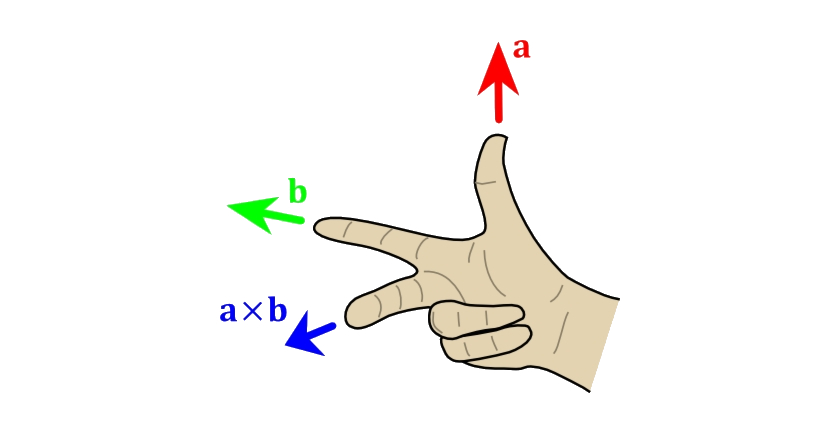
\includegraphics[width=\columnwidth]{img/manodestra.jpg}
\end{frame}



\begin{frame}
  \frametitle{Prodotto vettoriale (4)}
Vale la \emph{proprietà anticommutativa}:
\begin{center}
 $ \vec{a} \times \vec{b} = -\vec{b}\times\vec{a} $ 
\end{center}~\pause\\
In \emph{forma cartesiana} il prodotto vettoriale si calcola con:
\begin{center}
\colorbox{blue!30}{ $ \vec{a} \times \vec{b} = (a_y b_z - a_z b_y)\hat{i} + (a_z b_x -a_x b_z )\hat{j} + (a_x b_y - a_y b_x)\hat{k} $ }
\end{center}
\end{frame}


\begin{frame}
\frametitle{Prodotto scalare e vettoriale}

\begin{tabular}{rcc}
&\textbf{Prodotto scalare} & \textbf{Prodotto vettoriale} \\\rule{0pt}{4ex}
scrittura&$ \vec{a} \cdot \vec{b} $ & $ \vec{a}\times \vec{b} $ \\\rule{0pt}{3ex}
risultato&scalare $ c $ & vettore $ \vec{c} $ \\\rule{0pt}{3ex}
forma trigonometrica&$ c = ab\cos\theta $ & $ c = ab\sin\theta $ \\\rule{0pt}{4ex}
è nullo se&$ \theta = 90^\circ $ & $ \theta = 0^\circ $ \\\rule{0pt}{4ex}
forma cartesiana&$ c = a_x b_x + a_y b_y $ & $ \vec{c} = (a_y b_z - a_z b_y)\hat{i} $ \\\rule{0pt}{2ex}
&& $~~~ + (a_z b_x -a_x b_z )\hat{j} $ \\\rule{0pt}{2ex}
&&  $~~~~ + (a_x b_y - a_y b_x)\hat{k} $ \\
\end{tabular}

~

~

Attenzione: per il prodotto vettoriale, il vettore $ \vec{c} $ è perpendicolare al piano individuato da $ \vec{a} $ e $ \vec{b} $!
\end{frame}






\end{document}
